% region Filename parsing.
% Provides macros manipulating strings of tokens.
\RequirePackage{xstring}

% Store the jobname as a string with category 11 characters.
\edef\normaljobname{\expandafter\scantokens\expandafter{\jobname\noexpand}}
\StrBetween{\normaljobname}{hw-}{-q}[\homeworknumber]
\StrBehind{\normaljobname}{-q-}[\questionnumber]
% endregion

\documentclass[
  coursecode={MTHE 477},
  assignmentname={Homework \homeworknumber},
  studentnumber=20053722,
  name={Bryan Hoang},
  draft,
  % final,
]{
  ltxanswer%
}

\usepackage{bch-style}

\begin{document}
  \begin{questions}
    \setcounter{question}{\questionnumber}
    \addtocounter{question}{-1}
    \question[25]\
    \begin{parts}
      \part{}
      \begin{solution}
        Let \(\bar{X}^{n}\) denote the converted asymmetric source. By Shannon's source coding theorem, the minimum rate that can losslessly encode the source is the source entropy. If we can find the source's entropy, we can make \(R_{1}\) approach it in the limit for large \(n\) and thus determine the function.

        First, let's look at the distribution of \(\bar{X}^{n}\).
        \begin{align*}
          p_{\bar{X}}(1)             &= p_{X}(1) p_{\bar{X}|X}(1|1) + p_{X}(0) p_{\bar{X}|X}(1|0) \\
                                     &= \frac{1}{2}(1) + \frac{1}{2}(p)                           \\
                                     &= \frac{1}{2}(1 + p)                                        \\
          \Rightarrow p_{\bar{X}}(0) &= 1 - p_{\bar{X}}(1)                                        \\
                                     &=\frac{1}{2}(1 - p).
        \end{align*}
        Then the source entropy of \(\bar{X}^{n}\) is
        \begin{equation*}\label{eq:binary-entropy}
          H(\bar{X}) = H_{b}(\frac{1}{2}(1-p))
        \end{equation*}
        where \(H_{b}\) is the binary entropy function.

        With the constraint that the scheme yield an expected constraint of at most \(D\), we have that
        \begin{align*}
          Ed(X^{n},\hat{X}^{n})             &\le D                                              \\
          \Rightarrow Ed(X^{n},\bar{X}^{n}) &\le D\numberthis\label{eq:expected-distortion-bar}
        \end{align*}
        since the asymmetric source is losslessly encoded and decoded, meaning that no distorting occurs during those steps. It follows from~\eqref{eq:expected-distortion-bar} that
        \begin{align*}
          Ed(X^{n},\bar{X}^{n})                                                                                                                                                                                                                    &\le D                                  \\
          \sum_{x^{n}\in\X^{n}} \sum_{\bar{x}^{n}\in\bar{\X}^{n}} p_{X^{n}}(x^{n}) p_{\bar{X}^{n}|X^{n}}(\bar{x}^{n}|x^{n}) d(x^{n},\bar{x}^{n})                                                                                                   &\le D                                  \\
          \sum_{x^{n}\in\X^{n}} \underbrace{\biggl(\frac{1}{2}\biggr)^{n}}_{\because\ X^{n} \sim \text{Bernoulli}(\frac{1}{2})} \underbrace{\biggl(\frac{1}{n} \sum_{i=1}^{n} P(x_{i} \ne \bar{x}_{i})\biggr)}_{\text{\because\ Hamming distance}} &\le D
          \intertext{Since the flips during the conversion from the symmetric source to the asymmetric source are independent, we also have \(P(x_{i} \ne \bar{x}_{i}) = P(x_{i}=0,\bar{x}_{i}=1)=\frac{1}{2}p\). Thus, we have that}
          2^{n} \cdot \biggl(\frac{1}{2}\biggr)^{n} \cdot n \cdot \frac{1}{n} \cdot \frac{1}{2}p                                                                                                                                                   &\le D                                  \\
          \frac{1}{2}p                                                                                                                                                                                                                             &\le D.\numberthis\label{eq:inequality}
        \end{align*}
        From~\eqref{eq:binary-entropy}, the source entropy is bounded below by
        \begin{align*}
          H(\bar{X}) &= H_{b}(\frac{1}{2}(1-p))  & &\text{which is decreasing on \(p\in[0,1]\)} \\
                     &\ge H_{b}(\frac{1}{2} - D) & &\because~\eqref{eq:inequality}
        \end{align*}
        for \(0 \le D \le \frac{1}{2}\).

        For \(\frac{1}{2} \le D \le 1\), it's clear that the distortion constraint is still satisfied.

        Since we can make \(R_{1}\) approach the source entropy in the limit for large \(n\), we have
        \begin{equation*}
          \boxed{R_{1}(D) = \begin{cases}
              H_{b}(\frac{1}{2}-D), &0 \le D \le \frac{1}{2}, \\
              0,                    &\frac{1}{2} \le D \le 1.
            \end{cases}}
        \end{equation*}
      \end{solution}

      \part{}
      \begin{solution}
        For the distortion constraint to be satisfied, we need to have
        \begin{align*}
          Ed(X^{n},\hat{X}^{n})                                                                                                 &\le D                                                  \\
          \sum_{x^{n}\in\X^{n}} \biggl(\frac{1}{2}\biggr)^{n} \biggl(\frac{1}{n} \sum_{i=1}^{n} P(x_{i} \ne \hat{x}_{i})\biggr) &\le D
          \intertext{where \(P(x_{i} \ne \hat{x}_{i}) = \begin{cases}
                                                            \frac{1}{2}, &i \in \{1, \dotsc, nR_{2}\}   \\
                                                            0,           &i \in \{nR_{2}+1, \dotsc, n\}
                                                          \end{cases}\). Then}
          \frac{1}{2}(1-R_{2})                                                                                                  &\le D                                                  \\
          R_{2}                                                                                                                 &\ge 1-2D & &\forall D \in \biggl[0, \frac{1}{2}\biggr]
        \end{align*}
        For \(\frac{1}{2} \le D \le 1\), it's clear that the distortion constraint is still satisfied. Therefore,
        \begin{equation*}
          \boxed{R_{1}(D) = \begin{cases}
              1-2D, &0 \le D \le \frac{1}{2}, \\
              0,    &\frac{1}{2} \le D \le 1.
            \end{cases}}
        \end{equation*}
      \end{solution}

      \part{}
      \begin{solution}
        From theorem 5 in lecture, we have that
        \begin{equation*}
          R(D) = \begin{cases}
            1-H_{b}(D), &0 \le D \le \frac{1}{2}, \\
            0,          &\frac{1}{2} \le D \le 1.
          \end{cases}
        \end{equation*}
        \begin{answerfigure}
          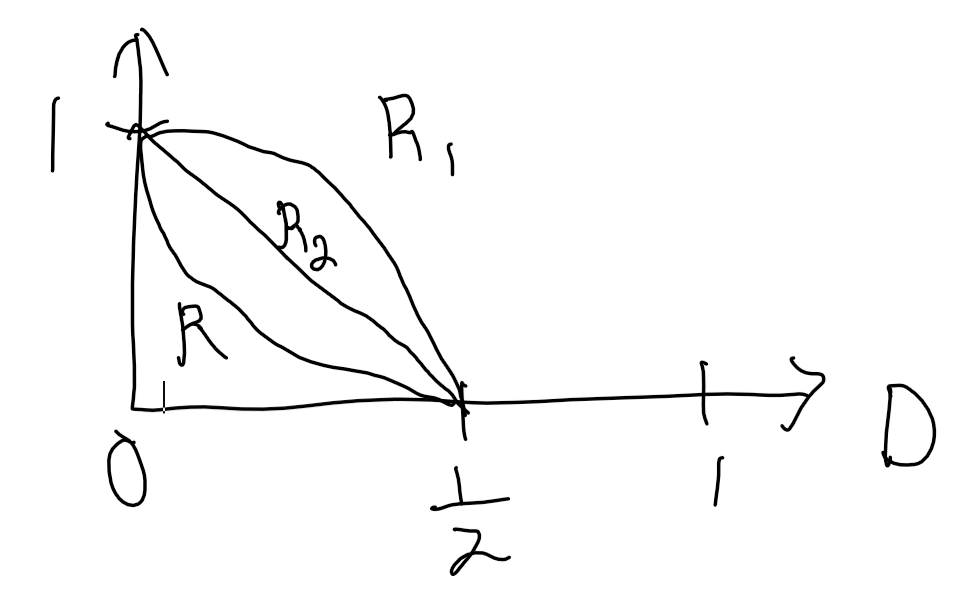
\includegraphics{img/q-3-c-graph.png}
          \caption{Plot of \(R_{1}(D), R_{1}(D)\), and \(R(D)\) on the same graph.}
        \end{answerfigure}
      \end{solution}
    \end{parts}
  \end{questions}
\end{document}
